
\documentclass[12pt,a4paper,openany]{book}

%Uporabljeni paketi
\usepackage{fancyhdr}
\usepackage{graphicx}
\usepackage{color}
\usepackage{xcolor}
\usepackage[slovene]{babel}



\usepackage[utf8]{inputenc}
\usepackage[pdftex,bookmarks=true]{hyperref}

%Velikost strani - dvostransko
\oddsidemargin 1.4cm
\evensidemargin 0.35cm
\textwidth 14cm
\topmargin 0.26cm
\headheight 0.6cm
\headsep 1.5cm
\textheight 20cm

%Nastavitev glave in repa strani
\pagestyle{fancy}
\fancyhead{}
\renewcommand{\chaptermark}[1]{\markboth{\textsf{Poglavje \thechapter:\ #1}}{}}
\renewcommand{\sectionmark}[1]{\markright{\textsf{\thesection\  #1}}{}}
\fancyhead[RE]{\leftmark}
\fancyhead[LO]{\rightmark}
\fancyhead[LE,RO]{\thepage}
\fancyfoot{}
\renewcommand{\headrulewidth}{0.0pt}
\renewcommand{\footrulewidth}{0.0pt}

\newtheorem{theorem}{Izrek}[section]
\newtheorem{lemma}[theorem]{Lemma}
\newtheorem{proposition}[theorem]{Proposition}
\newtheorem{corollary}[theorem]{Corollary}

\newenvironment{proof}[1][Proof]{\begin{trivlist}
\item[\hskip \labelsep {\bfseries #1}]}{\end{trivlist}}
\newenvironment{definition}[1][Definition]{\begin{trivlist}
\item[\hskip \labelsep {\bfseries #1}]}{\end{trivlist}}
\newenvironment{example}[1][Example]{\begin{trivlist}
\item[\hskip \labelsep {\bfseries #1}]}{\end{trivlist}}
\newenvironment{remark}[1][Remark]{\begin{trivlist}
\item[\hskip \labelsep {\bfseries #1}]}{\end{trivlist}}

\newcommand{\qed}{\nobreak \ifvmode \relax \else
      \ifdim\lastskip<1.5em \hskip-\lastskip
      \hskip1.5em plus0em minus0.5em \fi \nobreak
      \vrule height0.75em width0.5em depth0.25em\fi}

%********************************************

\begin{document}

% stran 1 med uvodnimi listi
\thispagestyle{empty} 

\begin{center}
{\large 
UNIVERZA V LJUBLJANI\\
FAKULTETA ZA RAČUNALNIŠTVO IN INFORMATIKO\\
}

 
\includegraphics[scale=0.2,keepaspectratio=true]{./pictures/uni_logo.png}


\vspace{1.5cm}
{\LARGE Daniel Rižnar, Uroš Kosič}\\

\vspace{2cm}
\textsc{\textbf{\LARGE 
Umetna inteligenca 2
}}

\vspace{2cm}
{ SEMINARSKA NALOGA}\\
{ POROČILO }\\

\vspace{2cm} 
{\Large Mentor: Martin Možina}

\vfill
{\Large Ljubljana, 2011}
\end{center}

\newpage

%********************************************

\renewcommand\thepage{} 
\tableofcontents 
\renewcommand\thepage{\arabic{page}}

\thispagestyle{empty}




\setcounter{page}{1}
\pagenumbering{arabic}

\chapter*{Povzetek}

\addcontentsline{toc}{chapter}{Povzetek}
Namen dokumenta je, predstaviti naše delo, ki se je izvajalo v sklopu vaj pri predmetu
 Porazdeljene inteligentne programske tehnologije. Cilj vaj je bil implementirati znanja
 in ideje, ki smo jih pridobili pri predmetu. Implementacija je v obliki agenta, ki sodeluje
 z drugimi agenti pri igranju igre Capture The Flag (CTF). Asistent pri predmetu nam je pripravil
 simulirano okolje agenta, v katerem se igra odvija.
\\
V tem dokumentu se bomo dotaknili problemov, kot so raziskovanje prostora z več agenti, sodelovanje med agenti, 
iskanje zastave, ter razne ofenzivne in defenzivne taktike pri sami igri.
\\
Pri raziskovanju prostora je cilj, podobno kot pri raziskovanju z enim samim agentom, minimizirati skupen porabljen čas.
 V našem primeru je cil, da agenti v čim krajšem času odkrijejo zastavo. Glavni problem, ki ga je potrebno rešiti v kontekstu
 raziskovanja z večimi agenti je izbira primernih smernic za posameznega agenta, tako da istočasno raziskujejo različne predele 
prostora. Tega smo se lotili tako, da vsak agent oceni ceno poti do ciljne točke in njen prispevek. Ob vsakem morebitnem srečanju 
pa si izmenjajo informacijo o prostoru, ki so jo do tistega trenutka pridobili.\\
\\
\\
Za oblikovanje tega dokumenta je bil uporabljen sistem \LaTeX.

\vspace{1.3cm}
\noindent
{\large \bf Ključne besede:}

\vspace{0.5cm}
\noindent
Agenti, sodelovanje, CTF, raziskovanje, algoritmi, AI.



%********************************************

\chapter{Opis naloge}
RPG (role-playing game) ali igra igranja vlog je izraz za igre, v katerih igralci prevzamejo vloge namišljenih likov, postavljenih v domišljijsko okolje. Bodisi z neposrednim igranjem, bodisi z opisovanjem njihovih dejanj nato igrajo te vloge v zgodbi, ki je lahko vnaprej začrtana ali pa nastaja sproti. Uspeh ali neuspeh njihovih dejanj določa dogovorjen sistem pravil konkretne igre. Velik problem je ravnotežje različnih likov, saj se v večini primerov izkaže, da imajo nekateri liki prednost pred ostalimi in lažje zmagujejo v neposrednih dvobojih.

Posamezna RPG igra ponuja izbiro med več različnimi bojevniki, vsak ima svoje prednosti in slabosti. V tem poglavju bomo opisali konkretne značilnosti naše igre in predstavili problem.

\section{Značilnosti igre}
V igri sodelujeta dva igralca, vsak s svojim bojevnikom. Bojno polje je plošča poljubne velikosti, razdeljena na kvadratno mrežo. Bojevnika izmenično izvajate v naprej definirane akcije. Cilj igre je pokončati nasprotnika, preden on pokonča tebe. Vsak bojevnik ima na izbiro v naprej določene akcije, ki jih opisuje tabela ~\ref{table:akcijeBojevnikov}. Posamezni bojevnik je opisan z atributi, ki jih podaja ~\ref{table:atributiBojevnikov}.


\begin{table}[ht] \caption{Akcije bojevnikov}
\centering
\begin{tabular}{cp{10cm}}
\hline\hline
Akcija & Opis Akcije \\ [0.5ex]
%heading 
\hline 
Move & Akcija pomeni premik v eno izmed štirih smeri (gor, dol, levo, desno). Vsak premik zahteva določeno količino energije.\\
Pass & Akcija pomeni počitek, bojevniku se ob počivanju poveča energija.\\
Fire & Strel s primarnim orožjem. Vsak strel pomeni zmanjšanje določene količine energije in zmanjšanje življenja nasprotnika. Škoda je delno odvisna tudi od naključja.\\ [1ex]
\hline %inserts single line
\end{tabular}
\label{table:akcijeBojevnikov} % is used to refer this table in the text
\end{table}

\begin{table}[ht] \caption{Atributi bojevnikov}
\centering
\begin{tabular}{cp{10cm}}
\hline\hline
Atribut & Opis Atributa \\ [0.5ex]
%heading 
\hline 
Life & Celo število, ki opisuje količino življenja ob začetku igre.\\
Speed & Hitrost, ki opisuje za koliko kock se bojevnik lahko premakne ob premikih.\\
Energy & Začetna energija bojevnika, ki jo lahko porabi za izvajanje akcij.\\ [1ex]
\hline %inserts single line
\end{tabular}
\label{table:atributiBojevnikov} % is used to refer this table in the text
\end{table}

\section{Bojevniki}
Za potrebe seminarske naloge, smo se omejili le na dva bojevnika - Tank in Vojak. 
Značilnosti obeh smo določili kot v tabeli ~\ref{table:bojevniki}. 
\begin{table}[ht] \caption{Značilnosti bojevnikov}
\centering
\begin{tabular}{ccccccc}
\hline\hline
Tip & Trpežnost & Domet & Hitrost & Obnavljanje & Varčnost  & Energija \\ [0.5ex]
%heading 
\hline 
Tank & boljša & boljši & višja & slabše & boljša & višja\\
Vojak & slabša & slabši & nižja & boljše & slabša & nižja\\ [1ex]
\hline %inserts single line
\end{tabular}
\label{table:bojevniki} % is used to refer this table in the text
\end{table}


\section{Opis problema}
Znan problem v RPG igrah je ravnotežje različnih likov, ki tekmujejo med seboj. Kljub različnim lastnostim, morajo imeti bojevniki enake možnosti za zmago v igri. Naša naloga je bila poiskati konkretne vrednosti atributov za zgoraj opisana bojevnika tako, da bosta igrala čim bolj izenačeno igro. Problem smo ločili na dva dela - simulacijo igranja in optimizacijo izenačenosti bojevnikov. Za simulacijo igranja smo uporabili \textit{minimax} algoritem. Za optimizacijo smo uporabili \textit{genetske algoritme} in jih primerjali s \textit{hill climbing}-om.

\chapter{Metode dela}
V tem poglavju bomo opisali uporabljene algoritme in načine izvajanja meritev. Na koncu poglavja bomo podali nekaj implementacijskih podrobnosti.

\section{Simulacija igranja}
Za simulacijo igranja igre smo uporabili algoritem \textit{minimax}. Z njim smo poskušali doseči, da igralca igrata čim bolj optimalno igro, tj. v danem trenutku izbereta najboljšo možno potezo.

Algoritem se uporablja za minimizacijo možne izgube, pri maksimizaciji možnega dobička. V naši igri igralca izmenjujeta poteze in poskušata izbrati najboljšo svojo potezo oz. maksimizirati svojo vrednost, posledično pa minimizirati nasprotnikovo. Tako glede na trenutno pozicijo identificiramo igralca MIN in MAX. Tisti ki je na potezi predstavlja igralca MAX, nasprotnik pa igralca MIN. 




\subsection{Zaznavanje prostora}
Zaznavanje prostora je določeno z parametri okolja.  Agent zaznava kvadraten del prostora z središčem
njegovega položaja. Agent ločuje med različnimi objekti v prostoru, kot so; zid, prazen prostor, nasprotnik, nasprotnikova baza,
nasprotnikova zastava, njegova zastava, njegova baza in član njegove skupine z njegovo ID številko.


\section{Akcije agenta}
Agent lahko vpliva na okolje z; svojim gibanjem, z pošiljanjem sporočil in lahko nosi zastavo svoje ekipe.

\subsection{Gibanje}
Agent se lahko vedno premakne v katerokoli od štirih smeri (gor, dol, levo in desno), ne glede na to,
kaj je takrat v tisti celici. V primeru da se želi premakniti v celico, ki je označena kot zid, izgubi
življenje in se vrne v bazo, kjer zopet začne z novim preiskovanjem. Podobno se zgodi tudi takrat, če
se premakne v celico, kjer je že eden od njegovih ali nasprotnikovih robotov. V tem primeru življenje izgubita oba.

\subsection{Pošiljanje sporočil}
Pošiljanje sporočil je omejeno z razdaljo med agenti. Trenutne nastavitve okolja omogočajo posredovanje sporočil
 le agentom, ki so znotraj vidnega polja. Sporočilo se pošlje s pomočjo ID številke agenta ki je v isti ekipi.
 Dolžina sporočila je omejena, prav tako pa so sankcionirani agenti, ki med seboj prekomerno komunicirajo.

\subsection{Manipulacija z zastavo}
Agent lahko pobere zastavo svoje ekipe, in jo odnese v svojo bazo. Če med vračanjem domov agent umre zaradi
kakršnega koli vzroka, se zastava v zadnje obiskani celici spusti na tla in ostali agenti potem ko jo najdejo,
nadaljujejo od tam naprej. Igra dopušča tudi možnost, da je na enkrat na zemljevidu postavljenih več zastav za eno ekipo.



\chapter{Problemi na katere smo naleteli}

\section{Raziskovanje}
Pri raziskovanju prostora je pomembno, da si agenti čimbolj razdelijo prostor, ki ga preiskujejo. Pomembno je tudi,
da preiščejo ves prostor, do katerega lahko pridejo (Dokler ne najdejo zastave).\\
\\
Razsikovanje je implementirano tako, da vse neobiskane celice oceni in nato izbere najboljšo. Ocena se izračuna na 
podlagi tega, koliko novih celic odkrijemo če obiščemo to pozicijo, ta ocena je skalirana z razdaljo te pozicije od 
trenutne pozicije. Majhen vpliv na oceno pa predstavlja bljižina zidu. Tem bližje kot smo zidu, tem manjša je ocena. 
Do najboljše pozicije agent izdela plan poti s pomočjo algoritma A*.\\
Ta strategija se je izkazala kot učinkovita, vendar se včasih izkaže, da na poti izpušča majhne kotičke, do katerih 
mora naknadno dostopati, po seveda veliko daljši poti. Rešitev za ta problem bi bila, če bi agenta prisilili, da raje 
izbira pot, ki je v ravni liniji.\\
Da se agenti, ki ne utegnejo komunicirati med sabo (zaradi prevelike razdalje), nebi očali za isto pot, je v samo 
hveristiko potrebno vnesti nek naključen člen. Ta vpliv pa mora biti seveda manjši od vseh ostalih. Ker je 
agentov veliko smo implementirali, tako da so nekateri agenti bolj podvrženi naklučju in nekateri manj.

\section{Iskanje poti do zastave}

V primeru, ko se zastava agentove skupine pojavi v njegovem vidnem polju ve katera je njegova ciljna celica, 
ni pa nujno da obstaja pot po raziskanem prostoru, do te celice. V primeru da pot obstaja, je problem trivialen 
in agent gere po zastavo. V primeru ko pa poti ni, pa je potrebno prostor nadaljne raziskati. Na sliki \ref{grupe}
 so z svetlejšo barvo označeni predeli, do katerih s trenutnim znanjem agent ne zna priti.\\
\begin{figure}[ht]
 \centering
 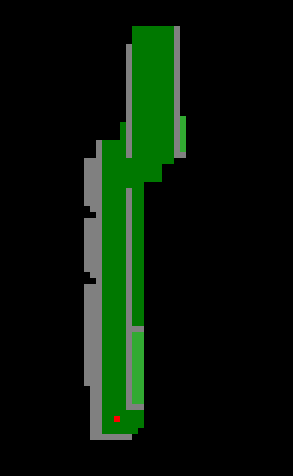
\includegraphics[width=7cm]{./pictures/Grupe.png}
 \caption[Agentova predstavitev sveta]{Agentova notranja predstavitev sveta}
 \label{grupe}
\end{figure}
\\
V naši implementaciji agenta se s slednjim problemom soočamo tako, da agent sledi zidu v levo ali desno stran. 
Tako so nekateri agenti levičarji in drugi desničarji, to se izračuna na podlagi njegove ID številke. Razdelitev 
agentov na desničarje in levičarje nam reši dve stvari, to da agenti ne sledijo isti poti. Ter dopušča možnost, 
da nek agent najde krajšo pot. Seveda vsem agentom, ki jih sreča na poti sporoči svoja spoznanja, tako da se lahko 
zgodi, da manjkajoči del zemljevida izve od drugih agentov in problem postane zopet trivialen.


\section{Prenos zastave v domačo bazo}

Ko agent pobere zastavo je njegova naloga, da jo prenese v bazo svoje skupine. Pri tem pa lahko
 naleti na agenta nasprotne ekipe, ki ga po vsej verjetnosti poizkušal ovirati na njegovi poti.
 Agentu ne preostane drugega, kakor da se mu umika. Vendar pa je gibanje agenta, ki nosi zastavo
 počasnejše od gibanja agenta, ki zastave nima. Tako da je v tem primeru situacija neizbežna. 
Pomagamo si lahko le tako, da agenti iste skupine ščitijo agenta z zastavo.\\
\\
Agent s pomočjo algoritma A*, naredi plan do baze in ga izvaja. Slika \ref{plan} prikazuje izdelan 
plan Agenta lahko ščitimo na dva načina. Prvi način je ta, da se z agentom, ki ne nosi zastave, 
poizkušamo zaleteti v  agenta nasprotne skupine. Tako ima naš agent z zastavo prosto pot. 
Drugi način pa je ta, da agent brez zastave le spremlja agenta, ki zastave nima. Ko se 
nasprotnikov agent zaleti v agenta z zastavo (ob tem seveda oba agenta izgubita življenje), 
tako lahko preživeli agent pobere zastavo in nadaljuje pot proti bazi. Odločili smo se za 
implementacijo drugega primera ščitenja agentov, saj je lažji in prav tako učinkovit.\\
\begin{figure}[ht]
 \centering
 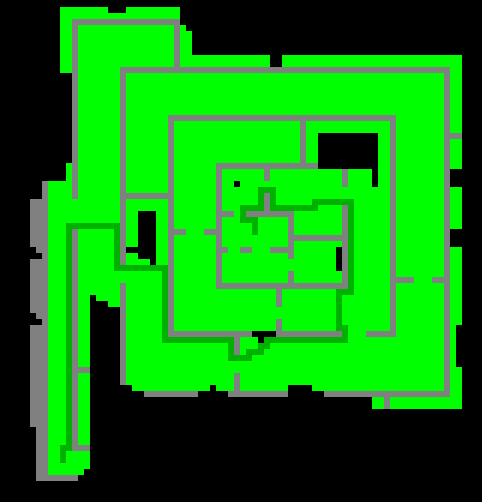
\includegraphics[width=10cm]{./pictures/plan.png}
 \caption[Izdelan plan]{Agentov plan od zastave do baze}
 \label{plan}
\end{figure}


\section{Srečanje z drugimi agenti}

Pri srečanju agenta iz iste ekipe, ob seveda prednosti komunikacije in posredovanja  medsebojnih informacij, 
obstaja nevarnost medsebojnega trka. To predstavlja nevarnost, da dva agenta izgubita življenje dva agenta.\\
\\
Ta problem smo rešili tako, da se agenti z nižjimi ID številkami ne ozirajo na agente z višjimi ID, jim pa 
sporočijo svojo namero gibanja. Tako se lahko agenti z višjo ID prilagodi agentu z nižjo. Izjema je primer, 
ko agent nosi zastavo, takrat ima ta agent prednost pred vsemi. Kako drugi agenti reagirajo na konfliktno 
stanje je odvisno od njihovega notranjega stanja. Če iščejo zastavo 

\subsection{Srečanje z agenti nasprotne ekipe}
Če se agent sreča z agentom nasprotne skupine pomeni, da je v njegovem vidnem polju. V primeru, da je kateri
izmed teh dveh agentov “nepazljiv” in se premakne v celico, kjer je drug agent, lahko pride do medsebojnega 
trka. Če agentova strategija ni usmerjena k uničevanju drugih agentov in s tem posledično tudi samega sebe, 
je edina logična pot ta, da se agenta poskušata zaobiti in s tem ohranita možnost iskanja vsak svoje zastave.\\
\\
Naši agenti so sprogramirani tako, da se poskušajo izogibati agentom nasprotne skupine. Ko se nasprotni
agent približa našemu agentu na razjo ene celice, se naš agent premakne v nasprotno smer od sovražnega agenta.
To pomeni, če naš agent vidi nasprotnika levo od svoje trenutne pozicije, se bo v naslenjem koraku premaknil desno,
če tam seveda ni kakšne druge ovire (stena, agent). Izjema je primer ko je agent varovan oziroma ima spremstvo,
torej nese zastavo proti bazi. V tem primeru, pa agent ne reagira na druge agente, temveč nese zastavo naravnost
proti bazi.


\subsection{Žrtvovanje agenta} 
Agenta ob trku oba izgubita življenje. Agent, ki izgubi življenje izgub vso informacijo, ki jo je do
tistega trenutka pridobil. Tako, da je v interesu celotne skupine, da se agent takim situacijam izogiba.
Vendar obstajajo situacije pri katerih, se izplača, da se agent žrtvuje. Primer take situacije je ko agent
nasprotne skupine nosi v svojo bazo. Vendar senzorika nam te informacije ne posreduje.\\
\\
V naši implementaciji agenta smo tako ubali strategijo, da agent, ki je svojo informacijo pred kratkim
(določeno s parametrom) predal naprej agentu z nižjim ID, ob morebitnem srečanju z nasprotnikom žrtvuje
življenje in upa, da mu je povzročil čim več nevšečnosti.
\newpage

%********************************************


\addcontentsline{toc}{chapter}{Seznam slik}
\addtocontents{toc}{\protect\vspace{-2ex}}
\listoffigures

\addcontentsline{toc}{chapter}{Seznam tabel}
\addtocontents{toc}{\protect\vspace{-2ex}}
\listoftables

\newpage





\end{document}

